\chapter{Metodi del gradiente}

I metodi del gradiente costituiscono una classe di metodi iterativi utilizzati per risolvere sistemi lineari della forma

\begin{equation*}
	A x = b,
\end{equation*}

dove $A \in \mathbb{R}^{n \times n}$ è una matrice simmetrica definita positiva (SPD).

Ricordiamo che una matrice simmetrica è definita positiva se vale la proprietà

\begin{equation*}
	v^T A v\ =\ (Av, v)\, >\, 0 \qquad \forall\ v \neq \{0\}\ \ .
\end{equation*}

Nota che la scrittura $v^T A v\ =\ (Av, v)$ è vera perché \textbf{A} è simmetrica, altrimenti se non lo fosse $(Av, v)$ si svilupperebbe come $(Av)^T v=v^T A^T v$, che non è chiaramente la stessa cosa.

\section{Formulazione variazionale del problema}

Sia $x = \phi$ la soluzione del sistema lineare $Ax = b$. 

Si può dimostrare che tale soluzione coincide con il minimo del funzionale quadratico

\begin{equation*}
	F(x) = \frac{1}{2}(Ax, x) - (b, x).
\end{equation*}

Per cui vale la relazione:

\begin{equation*}
	F(\phi)\ =\ \min_{x} F(x)\ \ .
\end{equation*}

\subsubsection{Dimostrazione}

Poiché $b = A\phi$, il funzionale può essere riscritto come
\begin{equation*}
	F(x)\ =\ \frac{1}{2}(Ax, x) \,-\, (A\phi, x)\ \ .
\end{equation*}

Valutando il funzionale nella soluzione esatta si ottiene

\begin{equation*}
	F(\phi)\ =\ \frac{1}{2}(A\phi, \phi)\, -\, (A\phi, \phi)\ =\ -\,\frac{1}{2}\,(A\phi, \phi)\ \ .
\end{equation*}

O, equivalentemente:

\begin{equation*}
	F(\phi)\, +\, \frac{1}{2}\,(A\phi, \phi)\ =\ 0\ \ .
\end{equation*}

Aggiungendo e sottraendo opportunamente termini, si può riscrivere $F(x)$ come

\begin{equation*}
	\begin{aligned}
		F(x)\ &=\ \frac{1}{2}(A\phi,\, \phi)\,-\,\color{blue}{(A\phi,\,  x)}\color{black}{\,+\,\underset{=0}{\underbrace{F(\phi)\,+\, \frac{1}{2}(A\phi,\,  \phi)}}\ =}\\
		&=\ F(\phi)\,+\, \frac{1}{2}(Ax,\,  x)\, \color{blue}{-\,\frac{1}{2}(A\phi, \, x)\, -\,\frac{1}{2}(A\phi,\,  x)}\color{black}{\,+\, \frac{1}{2}(A\phi,\,  \phi)\ =}\\
		&=\ F(\phi)\, +\, \frac{1}{2}\,(A(x-\phi),\, x)\, -\, \frac{1}{2}\,(A\phi, \,(x-\phi))\ =\\ 
		&=\ F(\phi)\, +\,\frac{1}{2}\,(A(x-\phi),\, x)\, -\, \frac{1}{2}\,(A(x-\phi),\, \phi)\ =\\
		&=\ F(\phi)\, +\, \frac{1}{2}\,(A(x-\phi), x-\phi) 
 .	\end{aligned}
\end{equation*}

Poiché $A$ è definita positiva, il termine $(A(x-\phi),\,  x-\phi)$ è sempre positivo per $x \neq \phi$. Ne segue che il minimo del funzionale è raggiunto esattamente per $x = \phi$.

\emph{Questo risultato mostra che la risoluzione del sistema lineare $Ax = b$ è equivalente alla minimizzazione del funzionale $F(x)$}.

\section{Interpretazione tramite errore}

Data una soluzione approssimata $x$, si possono definire diverse misure dell'errore:

\begin{equation}
	\label{errori gradiente}
	\begin{aligned}
		E_1(x)\ &=\ (\phi - x)^T\, (\phi - x)\ =\ \varepsilon^T\, \varepsilon\ , \\
		E_2(x)\ &=\ (b - Ax)^T\, (b - Ax)\ =\ r^T\, r\ , \\
		E_3(x)\ &=\ (\phi - x)^T\, (b - Ax)\ =\ \varepsilon^T\, A\, \varepsilon\ .
	\end{aligned}
\end{equation}

Indicando con $\varepsilon = \phi - x$ e osservando che $b - Ax = A\phi - Ax = A(\phi - x) = A\varepsilon$.

\emph{Tutte queste quantità sono nulle se e solo se $x = \phi$}.

%
%
\subsection{Relazione tra errore e funzionale}

Espandendo $E_3(x)$ si ottiene
\begin{align*}
	E_3(x) &= \phi^T b - \phi^T A x - x^T b + x^T A x \\
	&= \phi^T b + x^T A x - 2 x^T b\ \ .
\end{align*}

Utilizzando la definizione del funzionale $F(x)$, si ricava
\begin{equation*}
	E_3(x)\ =\ \phi^T b + 2F(x)\ .
\end{equation*}

Affinché l'errore si annulli nella soluzione esatta, deve valere
\begin{equation*}
	F(\phi)\ =\ -\frac{1}{2}\phi^T b = -\frac{1}{2}(A\phi, \phi)\ ,
\end{equation*}

che coincide con il valore minimo del funzionale.

\bigskip

In conclusione, la minimizzazione del funzionale $F(x)$ è completamente equivalente alla risoluzione del sistema lineare $Ax = b$, e fornisce la base teorica per lo sviluppo dei metodi iterativi basati sul gradiente.


\section{Metodi di discesa}

I metodi di discesa sono metodi iterativi che mirano a determinare il minimo del funzionale $F(x)$ costruendo una successione di approssimazioni $x^{(0)}, x^{(1)}, x^{(2)}, \dots$ a partire da una stima iniziale $x^{(0)}$.

L'idea fondamentale è che ogni nuova iterazione migliori la precedente, ovvero che il valore del funzionale decresca:
\begin{equation*}
	F\big(x^{(k+1)}\big) \leq F\big(x^{(k)}\big),
\end{equation*}
idealmente con disuguaglianza stretta.

Quando si raggiunge una configurazione tale che $Ax^{(k)} \approx b$, il processo può essere arrestato e $x^{(k)}$ viene considerata una buona approssimazione della soluzione.

\subsubsection{Struttura generale del metodo}

\begin{multicols}{2}
Il passaggio da $x^{(k)}$ a $x^{(k+1)}$ avviene tramite un processo in due fasi fondamentali:

\begin{enumerate}
	\item \textbf{Scelta della direzione di ricerca} $p^{(k)}$;
	\item \textbf{Scelta del passo} $\alpha_k$, che determina quanto muoversi lungo tale direzione.
\end{enumerate}

La nuova iterata è quindi definita come
\begin{equation*}
	x^{(k+1)}\ =\ x^{(k)}\, +\, \alpha_k \, p^{(k)}\  .
\end{equation*}

\begin{figure}[H]
	\centering
	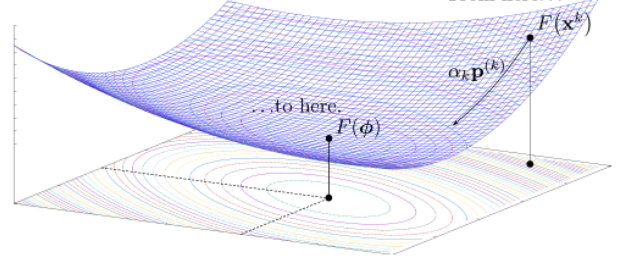
\includegraphics[width=8cm]{img/gradient1.png}
	\label{discesa}
	\caption{Visualizzazione delle grandezze definite.}
\end{figure}
\end{multicols}

Dal punto di vista matematico: $p^{(k)} \in \mathbb{R}^n$ è il vettore direzione;
$\alpha_k \in \mathbb{R}$ è un parametro scalare (step size).


\subsubsection{Scelta della direzione}

La scelta della direzione $p^{(k)}$ è cruciale per l'efficienza del metodo. Una scelta naturale per la direzione di discesa consiste nell’utilizzare il gradiente del funzionale. Infatti, la direzione in cui una funzione scalare varia più rapidamente è proprio quella del suo gradiente.

Si sceglie quindi come direzione di ricerca il negativo del gradiente:
\[\begin{aligned}
	p^{(k)}\ &=\ - \nabla\, F\big(x^{(k)}\big)\ =\ -\nabla\left[\frac{1}{2}(Ax^{(k)},\, x)\, -\, (b,\,x^{(k)})\right]\ =\\
	&=\ -\,\nabla\,\left[\frac{1}{2}\, x^{{(k)}^T}\,A\,x^{(k)}\, -\, x^{{(k)}^T}\, b\right]\ =\\
	&=\ -\, \left[\frac{1}{2} A x^{(k)} + \frac{1}{2} x^{{(k)}^T}\, A - b\right]\ \ .	
\end{aligned}\]

Poiché $A$ è simmetrica ($A = A^T$) , segue $\nabla F(x^{(k)}) = A x^{(k)} - b\,$ e, pertanto, la direzione di discesa diventa:
\begin{equation}
	\boxed{p^{(k)}\ =\ b\, -\, A x^{(k)}\ =\ r^{(k)}}\ \ ,
\end{equation}

dove $r^{(k)}$ è il \underline{residuo}, direzione lungo la quale il funzionale decresce maggiormente a partire da $x^{(k)}$.

%
%
%
\subsubsection{Scelta del passo}

Il parametro $\alpha_k$ viene scelto imponendo che il funzionale sia minimo lungo la direzione $r^{(k)}$, cioè:
\begin{equation}
	F\big(x^{(k+1)}\big) = \min_{\alpha_k} F\big(x^{(k)} + \alpha_k r^{(k)}\big).
\end{equation}

Per determinare tale valore, si impone la condizione di stazionarietà $\frac{d}{d\alpha_k} F\big(x^{(k+1)}\big) = 0$ e sostituendo $x^{(k+1)} = x^{(k)} + \alpha_k r^{(k)}$ nel funzionale si ottiene:
\begin{equation*}
	F\big(x^{(k+1)}\big)\ =\ \frac{1}{2}\, \left( A(x^{(k)} + \alpha_k r^{(k)}), \, x^{(k)}\, +\, \alpha_k r^{(k)} \right) 
	\, -\, \left( b, x^{(k)} + \alpha_k r^{(k)} \right)\ \ ,
\end{equation*}

ovvero, in forma matriciale:
\begin{equation*}
	F\big(x^{(k+1)}\big)\ =\ \frac{1}{2} (x^{(k)} + \alpha_k r^{(k)})^T A (x^{(k)}\, +\, \alpha_k r^{(k)}) 
	\, -\, (x^{(k)}\, +\, \alpha_k r^{(k)})^T\, b.
\end{equation*}

Sviluppando i termini si ottiene:
\begin{equation*}
	F\big(x^{(k+1)}\big)
	= \frac{1}{2} x^{(k)T} A x^{(k)}
	+ \alpha_k r^{(k)T} A x^{(k)}
	+ \frac{1}{2} \alpha_k^2 r^{(k)T} A r^{(k)}
	\quad - x^{(k)T} b - \alpha_k r^{(k)T} b.
\end{equation*}

Raccogliendo i termini:
\begin{equation*}
	F\big(x^{(k+1)}\big)
	= F\big(x^{(k)}\big)
	+ \alpha_k r^{(k)T} (A x^{(k)} - b)
	+ \frac{1}{2} \alpha_k^2 r^{(k)T} A r^{(k)}.
\end{equation*}

Poiché $r^{(k)} = b - A x^{(k)}$, segue:
\begin{equation*}
	F\big(x^{(k+1)}\big)
	= F\big(x^{(k)}\big)
	- \alpha_k r^{(k)T} r^{(k)}
	+ \frac{1}{2} \alpha_k^2 r^{(k)T} A r^{(k)}.
\end{equation*}

Imponendo la condizione di minimo:
\begin{equation*}
	\frac{d}{d\alpha_k} F\big(x^{(k+1)}\big)
	= - r^{(k)T} r^{(k)} + \alpha_k r^{(k)T} A r^{(k)} = 0,
\end{equation*}

da cui si ricava

\[\boxed{\,\alpha_k\ =\ \frac{r^{(k)T}\, r^{(k)}}{r^{(k)T}\, A\, r^{(k)}}\ =\ \frac{(r^{(k)},\, r^{(k)})}{(A r^{(k)},\, r^{(k)})}\, }\ \ .\]

La condizione di minimo del funzionale lungo la direzione di ricerca può essere riscritta in forma più compatta utilizzando la regola della derivazione composta. Infatti, si ha:

\begin{equation*}
	\frac{d}{d\alpha_k} F\big(x^{(k+1)}\big)
	\ =\
	\frac{dx^{(k+1)}}{d\alpha_k}
	\,\cdot\,
	\frac{dF\big(x^{(k+1)}\big)}{dx^{(k+1)}}
	\ =\ 0\ \ .
\end{equation*}

Dalla definizione dell'iterazione $x^{(k+1)} = x^{(k)} + \alpha_k r^{(k)}$, segue immediatamente che
\begin{equation*}
	\frac{dx^{(k+1)}}{d\alpha_k} = r^{(k)}.
\end{equation*}

D'altra parte, la derivata del funzionale rispetto alla variabile $x$ è il suo gradiente, quindi:
\begin{equation*}
	\frac{dF\big(x^{(k+1)}\big)}{dx^{(k+1)}} = \nabla F\big(x^{(k+1)}\big).
\end{equation*}

Ricordando che $\nabla F(x) = Ax - b = -r$, si ottiene:
\begin{equation*}
	\nabla F\big(x^{(k+1)}\big) = -r^{(k+1)}.
\end{equation*}

Sostituendo nella condizione di cui sopra, $r^{(k)} \cdot \big(-r^{(k+1)}\big) = 0$, segue la proprietà fondamentale
\begin{equation*}
	r^{(k)} r^{(k+1)} = 0 \qquad \rightarrow \quad r^{(k)}\perp r^{(k+1)} \ \ .
\end{equation*}

\subsubsection{Interpretazione}

La relazione precedente mostra che i residui di due iterazioni successive sono ortogonali tra loro.

Questa proprietà ha un significato geometrico molto importante: il passo $\alpha_k$ è scelto in modo tale che il nuovo punto $x^{(k+1)}$ sia il minimo del funzionale lungo la direzione $r^{(k)}$.

Di conseguenza:
\begin{itemize}
	\item il gradiente nel punto $x^{(k+1)}$ è ortogonale alla direzione seguita;
	\item poiché il gradiente è opposto al residuo, si ha che $r^{(k+1)}$ è ortogonale a $r^{(k)}$.
\end{itemize}

In altre parole, ogni iterazione elimina completamente la componente dell'errore lungo la direzione appena utilizzata.

Tuttavia, in generale non vale
\[
r^{(k)} r^{(j)} = 0 \quad \text{per } j \neq k \pm 1,
\]
cioè i residui non sono tutti mutuamente ortogonali, ma solo quelli consecutivi.

%
%
%
\subsection{Algoritmo del Steepest Descent Method}
Ecco lo pseudocodice che implementa il metodo, con ogni passaggio commentato:

\begin{lstlisting}[caption={Algoritmo del Steepest Descent Method}]
% Inizializzazione
x = x0;                % Stima iniziale
r = b - A * x;         % Residuo iniziale
	
% Iterazione fino a convergenza
while ||r|| > tolleranza
	
	% Calcolo del parametro alpha_k
	alpha = (r^T * r) / (r^T * A * r);
		
	% Aggiornamento della soluzione x_k -> x_{k+1}
	x = x + alpha * r;
		
	% Aggiornamento del residuo in funzione di x_{k+1}
	r = b - A * x;
	% potrebbe essere calcolato anche come 
	% b - A*x_k - alpha_k*A*r_k = r_k - alpha_k*A*r_k
end
\end{lstlisting}

\begin{itemize}
	\item \texttt{x0}: Stima iniziale della soluzione.
	\item \texttt{r}: Residuo iniziale, calcolato come \(\mathbf{b} - \mathbf{A} \mathbf{x}\).
	\item \texttt{alpha}: Parametro di passo calcolato come \(\frac{\mathbf{r}^T \mathbf{r}}{\mathbf{r}^T \mathbf{A} \mathbf{r}}\).
	\item \texttt{while ||r|| > tolleranza}: Iterazione finché il residuo non scende sotto una soglia prefissata.
	\item \texttt{x = x + alpha * r}: Aggiornamento della soluzione lungo la direzione del residuo.
	\item \texttt{r = b - A * x}: Aggiornamento del residuo dopo ogni iterazione.
\end{itemize}


%
%
%
\subsection{Interpretazione geometrica}

Data l'eq.(\eqref{errori gradiente}), dove \(\mathbf{\epsilon} = \mathbf{\phi} - \mathbf{x}\), se espandiamo \(\mathbf{\epsilon}\) in termini degli autovettori di \(\mathbf{A}\), $\mathbf{\epsilon} = \mathbf{U} \mathbf{z}$, dove \(\mathbf{U}\) è la matrice ortogonale degli autovettori e \(\mathbf{z}\) è il vettore dei coefficienti, otteniamo:

\begin{equation*}
	E_3(\mathbf{z})\ =\  (\mathbf{U} \mathbf{z})^T\, \mathbf{A}\, \mathbf{U} \mathbf{z}\ =\ \mathbf{z}^T \mathbf{U}^T\, \mathbf{A}\, \mathbf{U} \mathbf{z}\ =\ \mathbf{z}^T\, \mathbf{\Lambda}\, \mathbf{z},
\end{equation*}

con \(\mathbf{\Lambda}\) matrice diagonale degli autovalori \(\lambda_i\) di \(\mathbf{A}\).

\subsubsection{Iperellissoidi e autovalori}

L’equazione \eqref{eq:errore3} può essere riscritta come: $E_3(\mathbf{z}) = \lambda_1 z_1^2 + \lambda_2 z_2^2 + \dots + \lambda_n z_n^2$ .

I luoghi a errore costante sono rappresentati da iperellissoidi i cui semiassi sono legati agli autovalori di \(\mathbf{A}\):

\begin{equation*}
	r_i = \sqrt{\frac{E_3(\mathbf{z})}{\lambda_i}}.
\end{equation*}

La soluzione esatta \(\mathbf{\phi}\) corrisponde al centro degli iperellissoidi (dove \(E_3(\mathbf{z}) = 0\)).

\subsubsection{Visualizzazione geometrica}
Esempio tridimensionale (\(n=3\)) di iperellissoide.

Il metodo di discesa sposta \(\mathbf{x}^{(k)}\) sulla superficie $F(x)$ lungo la direzione di massima pendenza $r^{(k)}$ perpendicolare a $F(x^{(k)})$ fino al punto $x^{(k+1)}$ dove il funzionale assume il suo minimo valore lungo la direzione di spostamento.

Siccome vale l'ortogonalità dei residui successivi $r^{(k)}\perp r^{(k+1)}$, implica che, al passo \(k+1\), la direzione di discesa \(\mathbf{r}^{(k+1)}\) è perpendicolare all’iperellissoide corrispondente a $F(\mathbf{x}^{(k+1)})$ oltre che a $r^{(k)}$.

\begin{multicols}{2}
	
	\begin{figure}[H]
		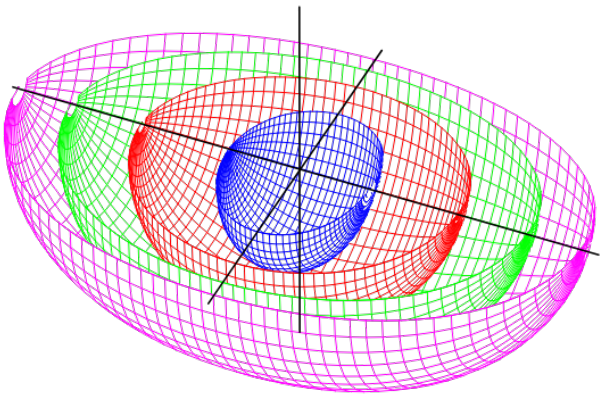
\includegraphics[width=6cm]{img/gradient2.png}
		\label{Ellissoidi}
		\caption{Visualizzazione degli ellissoidi per n=3}
	\end{figure}
	
	\begin{figure}[H]
		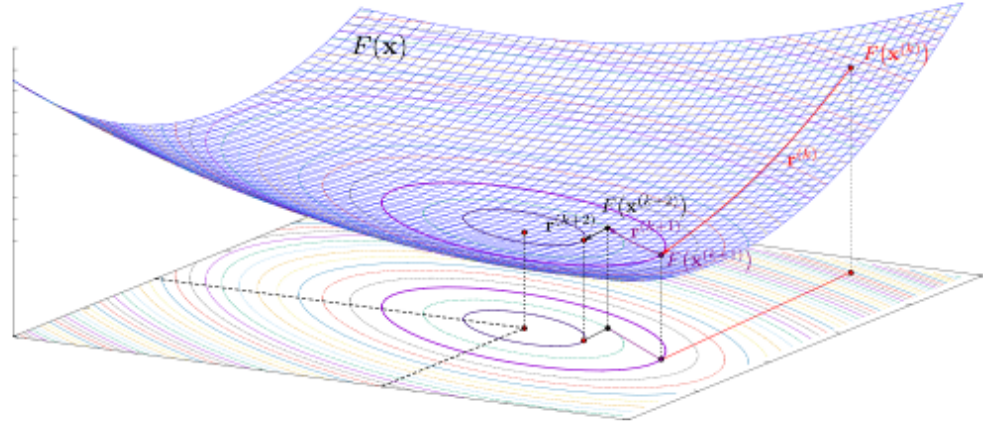
\includegraphics[width=7.5cm]{img/gradient3.png}
		\label{Discesa}
		\caption{Visualizzazione della discesa}
	\end{figure}
	
\end{multicols}
.

\begin{figure}[H]
	\centering
	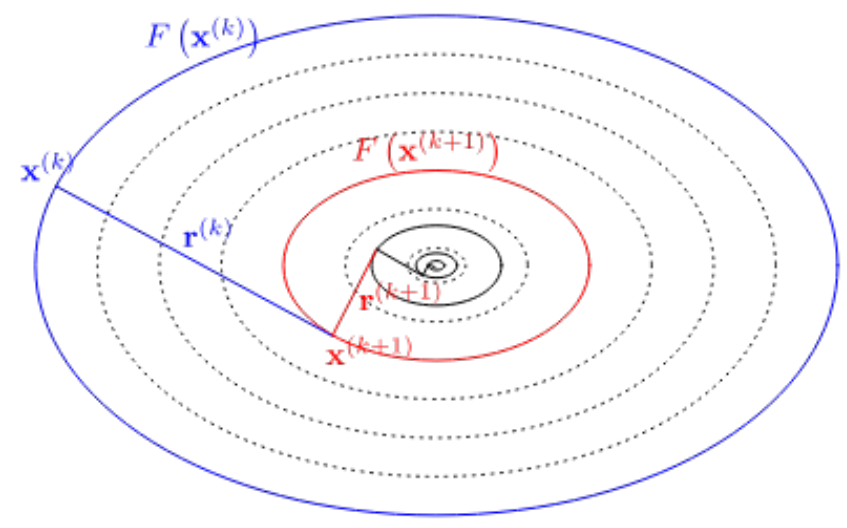
\includegraphics[width=9cm]{img/gradient4.png}
	\label{Gradient fatto bene}
	\caption{Metodo dello \emph{steepest descent} visualizzato nella sua totalità}
\end{figure}


\subsubsection{Condition number e convergenza}
Se la matrice \(\mathbf{A}\) ha numero di condizione \(\kappa(\mathbf{A}) = 1\) (cioè tutti gli autovalori sono uguali), gli iperellissoidi degenerano in ipersfere e il metodo converge in una sola iterazione, indipendentemente dal guess iniziale.

\begin{equation*}
	\kappa(\mathbf{A}) = \frac{|\lambda_{\text{max}}(\mathbf{A})|}{|\lambda_{\text{min}}(\mathbf{A})|}
\end{equation*}

\begin{multicols}{2}
\begin{figure}[H]
	\centering
	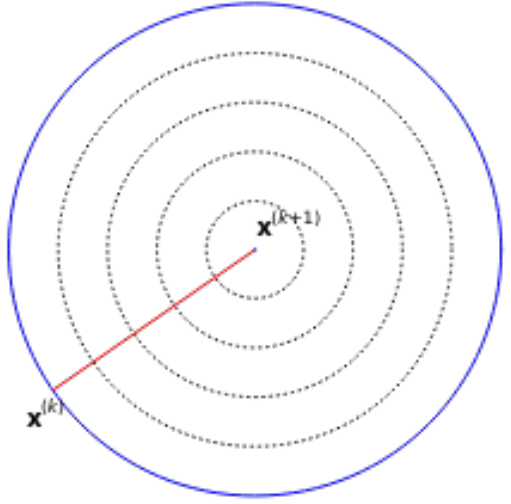
\includegraphics[width=5cm]{img/gradient5.png}
	\label{concentrici}
	\caption{Caso in cui gli iperellissoidi degenerano in ipersfere}
\end{figure}

\vspace{1cm}
\begin{figure}[H]
	\centering
	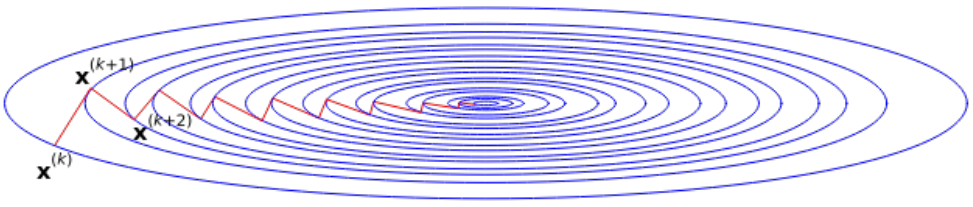
\includegraphics[width=7cm]{img/gradient6.png}
	\label{discesa lenta}
	\caption{Caso di matrice malcondizionata, che converge lentamente}
\end{figure}
\end{multicols}


Se gli autovalori sono raggruppati in un intervallo ristretto, la convergenza è veloce. Al contrario, se gli autovalori sono molto spaziati (matrice mal condizionata), la convergenza è lenta.

Se $\lambda_1 \gg \lambda_2$, l'iperellissoide è molto allungato lungo la direzione corrispondente a $\lambda_1$.
Il metodo di discesa "oscilla" tra le direzioni principali, rallentando la convergenza, come si vede in fig.(\ref{discesa lenta}).


%
%
%
\section{Conjugate Gradient Method}

Il metodo di Steepest Descent può essere lento, soprattutto per matrici mal condizionate, nel senso che può tornare spesso a muoversi in direzioni già usate in step precedenti. 

Il \underline{\emph{Conjugate Gradient Method}} è un algoritmo più efficiente che sfrutta direzioni di ricerca linearmente indipendenti.
L'algoritmo è simile a quello di Steepest Descent, ma la direzione di ricerca $\mathbf{p}^{(k)}$ è aggiornata come:

\begin{equation*}
	\mathbf{p}^{(k)} = \mathbf{r}^{(k)} + \beta_k \mathbf{p}^{(k-1)},
\end{equation*}

dove $\beta_k$ è scelto per garantire l'$\mathbf{A}$-ortogonalità:
$(\mathbf A \mathbf p^{(k-1)}, \mathbf p^{(k)}) = \mathbf{p}^{(k)^T} \mathbf{A} \mathbf{p}^{(k-1)} = 0$ .


\subsubsection{Calcolo di $\beta_k$ e del passo $\alpha_k$}

Imponendo la condizione di coniugazione, si ottiene:

\[
(\mathbf A \mathbf p^{(k-1)}, \mathbf{r}^{(k)} + \beta_k \mathbf{p}^{(k-1)})\ =\ 0
\]

\begin{equation*}
	\beta_k = -\frac{\mathbf{r}^{(k)^T} \mathbf{A} \mathbf{p}^{(k-1)}}{\mathbf{p}^{(k-1)^T} \mathbf{A} \mathbf{p}^{(k-1)}}.
\end{equation*}

L'insieme di direzioni di ricerca $\mathbf p^{(k)}$ così ottenuto formano un insieme di vettori linearmente indipendenti.

Il parametro \(\alpha_k\) è scelto per minimizzare \(F(\mathbf{x}^{(k+1)})\) lungo \(\mathbf{p}^{(k)}\):

\[\begin{aligned}
F(\mathbf{x}^{(k+1)})\ &=\ 
\frac{1}{2}\, (\mathbf A (\mathbf x^{(k)}+\alpha_k \mathbf p^{(k)}),\, (\mathbf x^{(k)}+\alpha_k \mathbf p^{(k)}))\, -\, (\mathbf b, \, (\mathbf x^{(k)}+\alpha_k \mathbf p^{(k)}))\ =\\
&=\ F(\mathbf x^{(k)})\, -\, \alpha_k \mathbf p^{(k)^T} \mathbf r^{(k)}\, +\, \frac{1}{2}\alpha_k^2 \mathbf{p}^{(k)^T} \mathbf A \mathbf p^{(k)}\ \ ,
\end{aligned}\]

\[
\frac{d\, F(\mathbf x^{(k+1)})}{d\, \alpha_k}\ =\ 0
\qquad \rightarrow \qquad
-\, \mathbf p^{(k)^T} \mathbf{r}^{(k)}\, +\, \alpha_k \mathbf{p}^{(k)^T} \mathbf A \mathbf p^{(k)}\ =\ 0\ \ ,
\]

\begin{equation*}
	\alpha_k = \frac{\mathbf{p}^{(k)^T} \mathbf{r}^{(k)}}{\mathbf{p}^{(k)^T} \mathbf{A} \mathbf{p}^{(k)}}\ =\ 
	\frac{(\mathbf{r}^{(k)},\, \mathbf{p}^{(k)})}{(\mathbf{A} \mathbf{p}^{(k)},\, \mathbf{p}^{(k)})}\ \ .
\end{equation*}


\subsection*{Pseudocodice del Conjugate Gradient Method}

\begin{lstlisting}[caption={Implementazione del CGM}]
% Inizializzazione
x = x0;                % Stima iniziale
r = b - A * x;         % Residuo iniziale
p = r;                 % Direzione iniziale
k = 0;                 % Contatore iterazioni
		
% Iterazione fino a convergenza
while |r| > tolleranza
	% Calcolo di alpha_k
	alpha = (p^T * r) / (p^T * A * p);
			
	% Aggiornamento della soluzione x_k -> x_{k+1}
	x = x + alpha * p;
			
	% Nuova direzione del residuo r_{k+1}
	r_new = r - alpha * A * p;
			
	if |r| < tollorenza
		end
			
	% Calcolo di beta_{k+1}
	beta = (r_new^T * A * p) / (p^T * A * p);
			
	% Aggiornamento della direzione di ricerca p^k -> p^{k+1}
	p = r_new + beta * p;
			
	% Preparazione per la prossima iterazione
	r = r_new;
	k = k + 1;
end
\end{lstlisting}


\begin{itemize}
	\item \texttt{x0}: Stima iniziale della soluzione.
	\item \texttt{r}: Residuo iniziale, $\mathbf{r}^{(0)} = \mathbf{b} - \mathbf{A} \mathbf{x}^{(0)}$.
	\item \texttt{p}: Direzione di ricerca inizializzata come il residuo.
	\item \texttt{alpha}: Parametro di passo calcolato come $\alpha_k = \frac{\mathbf{p}^{(k)^T} \mathbf{r}^{(k)}}{\mathbf{p}^{(k)^T} \mathbf{A} \mathbf{p}^{(k)}}$.
	\item \texttt{beta}: Parametro di coniugazione calcolato come $\beta_k = \frac{\mathbf{r}^{(k+1)^T} A\mathbf{p}^{(k)} }{ \mathbf{p}^{(k)^T} A\mathbf{p}^{(k)}}$.
\end{itemize}

---

\subsubsection{Proprietà del metodo}
Il Conjugate Gradient Method gode di proprietà fondamentali:
\begin{itemize}
	\item \textbf{Ortogonalità dei residui}: $\mathbf{r}^{(i)^T} \mathbf{r}^{(j)} = 0$ per $i \neq j$.
	\item \textbf{Coniugazione delle direzioni}: $\mathbf{p}^{(i)^T} \mathbf{A} \mathbf{p}^{(j)} = 0$ per $i \neq j$.
	\item \textbf{Convergenza in $n$ iterazioni}: Per un sistema di dimensione $n$, il metodo converge esattamente alla soluzione in al massimo $n$ passi (a meno di errori di arrotondamento).
	\item \textbf{Efficienza}: Ogni iterazione richiede una sola valutazione del prodotto matrice-vettore $\mathbf{A} \mathbf{p}^{(k)}$.
\end{itemize}

Si nota anche che per $k\in [0,\, n]$ e per $\ell\in [0,\, n-k-1]$ si verifica:

\[
\begin{aligned}
	(\mathbf r^{(k+\ell+1)},\, \mathbf r^{(k)})\ &=\ (\mathbf r^{(k+\ell)}\, -\, \alpha_{k+\ell}\mathbf A \mathbf p^{(k+\ell)}, \ \mathbf r^{(k)})\ =\\
	&=\ \mathbf r^{(k)^T} \mathbf r^{(k+\ell)}\, -\, \frac{\mathbf p^{(k+\ell)^T} \mathbf r^{(k+\ell)}}{\mathbf p^{(k+\ell)^T} \mathbf A \mathbf p^{(k+\ell)}} \mathbf r^{(k)^T} \mathbf A \mathbf p^{(k+\ell)}\ =\\
	& =\ \mathbf r^{(k)^T} \mathbf r^{(k+\ell)}\, -\, 
	\mathbf r^{(k+\ell)^T} \mathbf r^{(k)}\,
	\frac{\mathbf p^{(k+\ell)^T} \mathbf A \mathbf p^{(k+\ell)}}{\mathbf p^{(k+\ell)^T} \mathbf p^{(k+\ell)}} \ =\\
	& =\ 0
\end{aligned}
\]

Il residuo $\mathbf{r}^{(k+1)}$ è ortogonale a tutti i $\mathbf{r}^{(j)}$ precedenti, quindi $\mathbf{r}^{(n)} = 0$ e $\mathbf{x}^{(n)} = \mathbf{\phi}$ (soluzione esatta).

Le direzioni $\mathbf{p}^{(k)}$ sono linearmente indipendenti e $\mathbf{A}$-ortogonali, garantendo la convergenza rapida.


